\documentclass[letterpaper, twoside, 12pt,memoire]{thETS}
\interdisplaylinepenalty=2500
\usepackage{amsmath}
\usepackage{amsfonts}
\usepackage{amssymb}
\usepackage[utf8]{inputenc}
\usepackage{graphicx}
\usepackage{color}
\usepackage[T1]{fontenc}
\usepackage{subfigure}
\usepackage{setspace}
\usepackage{todonotes}
\usepackage{varwidth}
\usepackage[round]{natbibETS}
%\usepackage{url}

\newcommand{\LT}[1]{%
	{
	\todo[inline,color={red!33!green!33!blue!33}]{%
	\textbf{[LT]:}~#1}
	}}
	
\newcommand{\SC}[1]{%
	{
	\todo[inline,color={red!100!green!33}]{%
	\textbf{[SC]:}~#1}
	}}

\newcommand{\ltCodec}{logiciel de référence H.264/AVC JM}
\newcommand{\fig}[1]{figure~\ref{#1}}
\newcommand{\sect}[1]{section~\ref{#1}}
\newcommand{\ang}[1]{(\textit{#1})}

\begin{document}
\begin{chapter}{Résultats et analyse}
Au chapitre précédent, nous avons présenté les concepts théoriques des
nouvelles approches sélectives proposées, basées sur le MCB et le SDMCB \SC{On
utilise des acronymes français ou anglais pour cela? }. Dans ce chapitre, nous
faisons état des essais pratiques réalisés pour valider les gains réalisables à
l'aide de ces approches dans des conditions de vidéo mobile. Nous démontrons,
non seulement l'efficacité des approches sélectives proposées, mais aussi leur
supériorité par rapport à l'approche de dissimulation utilisée par le décodeur
inclus avec le \ltCodec.

Nous débutons par présenter nos hypothèses de validation à la section
\ref{sec-Hypotheses-validation}. Nous expliquons ensuite, à la section
\ref{sec-bancEssai}, les composantes de notre banc d'essai utilisées pour créer
notre jeu de tests. Dans le but de valider nos hypothèse sur le décodeur, les
taux de succès observés lors du décodage d'une séquence erronnée sont présentées
à la section \ref{sec-ResilienceDecodeur} \SC{je ne parle pas de probabilité car
c'est un événement mesuré, pas théorique}. Un succès sera considéré lorsque le
décodeur retournera une image sans planter\SC{trouver mieux que planter}.
Finalement, à la section \ref{sec-ApprocheSelective}, nous présentons les
résultats obtenus de l'application de nos algorithmes de détection et
dissimulation d'erreurs sur les images décodées.


\begin{section}{Hypothèses de validation}
\label{sec-Hypotheses-validation}

Débutons par énumérer les hypothèses faites dans le cadre de nos
expérimentations. À la \fig{fig-726}, nous présentons, à titre d'exemple, des
trames issues de la $726^{\text{e}}$ sous-séquence de notre jeu de tests
(expliqué plus en détail à la section suivante).  L'image erronée
\subref{fig-726-bad} correspond au résultat obtenu par le décodage d'une tranche
corrompue.

\begin{figure}[htb]
\fbox{\begin{varwidth}{\textwidth}\centering
\subfigure[Trame précédente]{
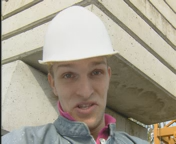
\includegraphics[width=0.46\linewidth]{images/prevForeman.png}
\label{fig-726-prev}
}
\subfigure[Trame erronée]{
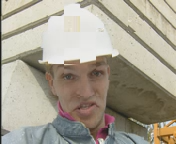
\includegraphics[width=0.46\linewidth]{images/badForeman.png}
\label{fig-726-bad}
}
\subfigure[Dissimulation par tranche calquée]{
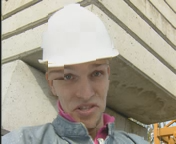
\includegraphics[width=0.46\linewidth]{images/fcForeman.png}
\label{fig-726-sc}
}
\subfigure[Trame de référence]{
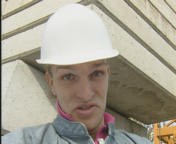
\includegraphics[width=0.46\linewidth]{images/perfForeman.png}
\label{fig-726-perf}
}
\end{varwidth}}
\caption{Les trames résultantes de la sous-séquence \#726 du jeu de tests
(Séquence~: Foreman, QP=16 BER=0.0008, FMO=Dispersé)}
\label{fig-726}
\end{figure}
\SC{pour la figure 1, il me semble que tu ne peux pas mettre les descriptions
dans les figures et il fait les mettre dans la description globale de la figure}

La trame qui précède l'erreur \subref{fig-726-prev} ne contient
jamais d'erreurs, une hypothèse posée aussi par~\citep{Superiori2007}. Nous
aurons recours à cette trame comme source de contenu pour la dissimulation
d'erreurs de la trame \subref{fig-726-bad}. La trame \subref{fig-726-sc} est
celle reconstruite à l'aide du calquage de la tranche de la trame précédente
\subref{fig-726-prev}. Cette trame représente la solution d'un décodeur moderne,
ce à quoi nous allons comparer nos dissimulations. La figure
\subref{fig-726-perf} est la trame de référence, qui n'a pas subit l'encodage.
C'est la trame que nous utilisons pour mesurer le PSNR.
\SC{mettre toutes tes hypothèses ici}. 
\end{section}

\begin{section}{Description du banc d'essai}
\label{sec-bancEssai}
Afin de valider notre notre approche de détection et de dissimulation vidéo,
nous avons construit un banc d'essai constitué d'un grand nombre de\SC{il me
semble que la phrase d'avant n'avait pas de sens. il me semble que tu n'étudie
pas tes hypothèses, enfin ce n'est pas le but premier du banc d'essaie. De plus
du n'étudie pas tes hypothèses sur la détection de la vraisemblance de régions
d’images. C'est quoi une détection de la vraisemblance? On fait une détection ou
on évalue la vraisemblance mais il me semble qu'on ne fait pas une détection de
la vraisemblance} séquences vidéos encodées à divers débits et soumises à des
taux d'erreurs similaires à ceux proposés dans l'ouvrage
\citep{Stockhammer2003}. Ces erreurs découlent des conditions difficiles de
transport de séquences vidéo H.264 vers des appareils évoluant sur des réseau
mobiles.

\begin{figure}[htb] \fbox{ \centering
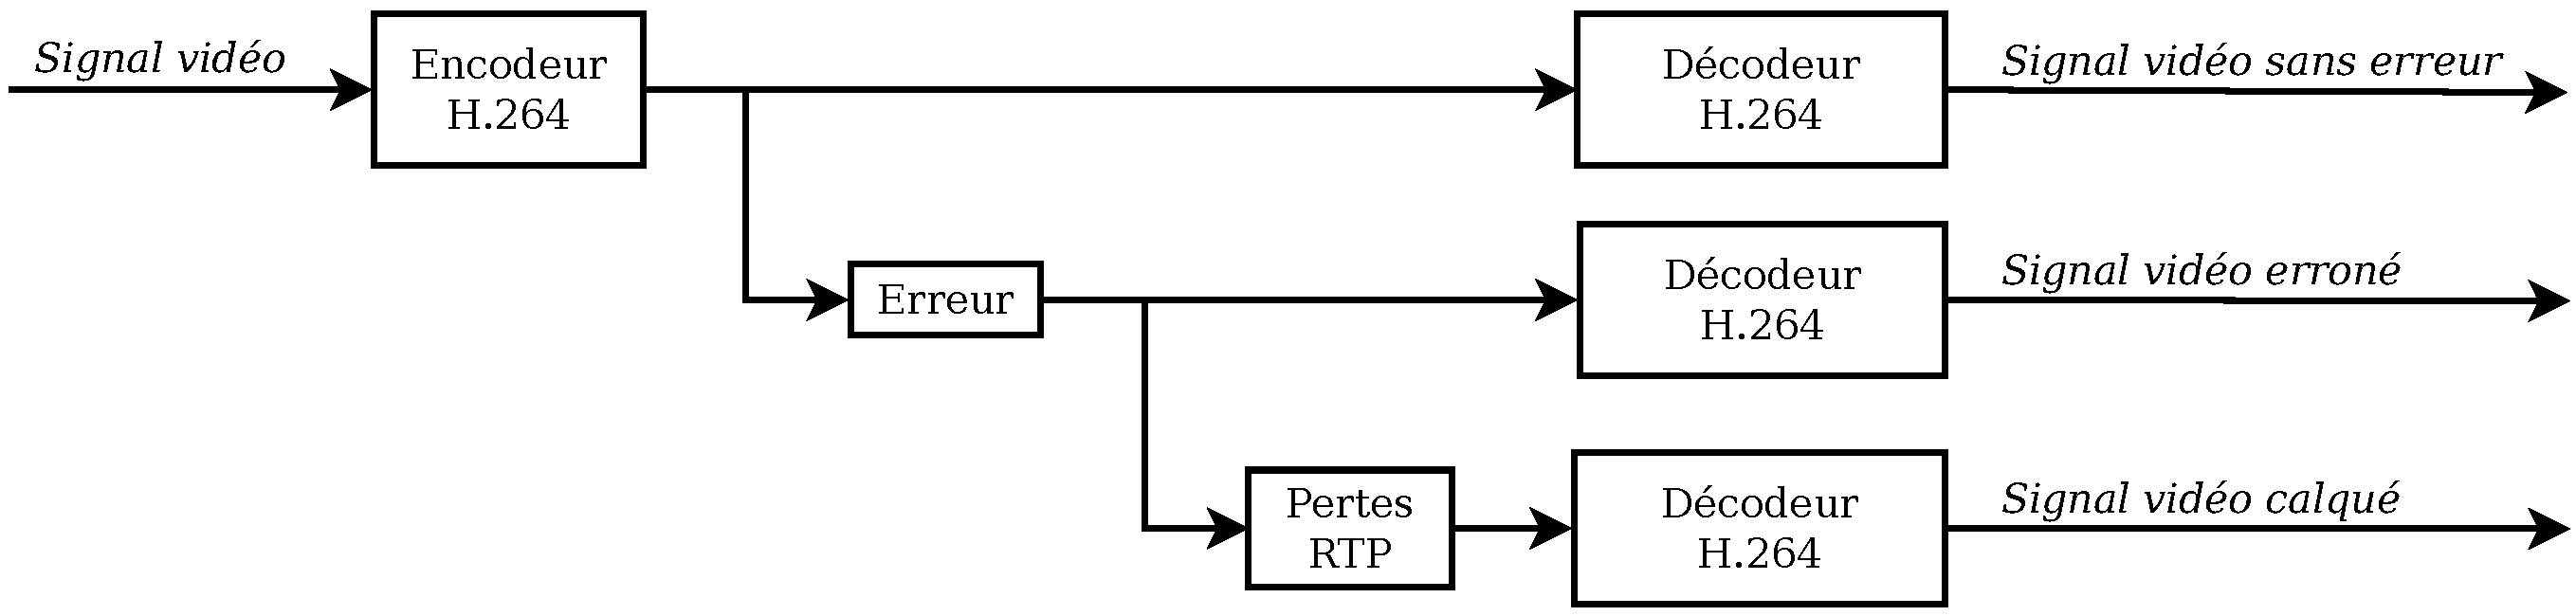
\includegraphics[width=0.97\linewidth]{images/EncoderDecoder.pdf} }
\caption{Diagramme des étapes du banc d'essai}
\label{fig-EncoderDecoder}
\end{figure}

Nous présentons, à la \fig{fig-EncoderDecoder}, les étapes de notre banc
d'essai. Nous y observons qu'un signal vidéo est encodé, transmis, puis décodé
trois fois. La première opération de décodage décode les données sans que
celles-ci soient exposées à l’erreur. Cette étape est cruciale afin de
déterminer la dégradation visuelle engendrée par l’encodage du signal \SC{on
mesure vraiment l'effet de l'encodage ou bien ça sert plutôt de référence pour
mesurer les erreurs de transport}. Dans la seconde opération, la séquence
encodée est sujette à un motif d’erreur binaire \ang{Bit Error Pattern}
gaussien. Les données corrompues sont envoyées au décodeur. S’il réussit à les
décoder, celles-ci sont conservées, sinon la sous-séquence est rejetée. En
dernier lieu, la sous-séquence corrompue est analysée par un module de détection
de pertes RTP \ang{RTP loss}. Celui-ci identifie et retire les paquets RTP
corrompus. Les données résultantes de l’analyse de pertes RTP sont décodées.
Lorsque le décodeur s'aperçoit d'un paquet manquant, il utilise une approche de
dissimulation d’erreurs,  en remplaçant, par exemple, la tranche manquante par
son équivalent dans la trame précédente\footnoteETS{Dans cet ouvrage,
\textit{slice copy} a été utilisé au détriment de \textit{motion copy}, car
aucune implémentation fonctionnelle de \textit{motion copy} était disponible.
Nous avons eux des problèmes lors de l'utilisation de \textit{motion copy} avec
les versions~15.1 à 16.2 du décodeur inclus dans le \ltCodec. Ces problèmes sont
connus et confirmés par plusieurs forums internet et catalogués dans le logiciel
de suivi de problèmes Mantis relié au \ltCodec~\citep{BUG}. Quoique notre
ouvrage est aussi compatible avec \textit{motion copy}, c'est pour cette raison,
que nous avons testé uniquement avec \textit{slice copy}.} (\textit{slice copy},
traduit dans cet ouvrage par la locution tranche calquée).

Les séquences sont encodées et décodées à l'aide de la version~16.2 du
\ltCodec~\citep{JM}. Ce dernier, n'étant pas un produit commercial, a pour
objectif principal la démonstration de nouvelles fonctionnalités visant la norme
H.264. Notre banc d'essai est constitué de sous-ensembles de quatre trames
consécutives commençant à un emplacement aléatoire dans diverses séquences
vidéos. Ces sous-ensembles débutent par une trame \textit{intra} et trois trames
\textit{inter} (IPPP). Nous retenons cinq sous-ensembles pour chaque séquence de
résolution QCIF contenue dans l'ensemble de séquences de référence de
l'Université de l'Arizona~\citep{YUV}.
\LT{Définir QCIF dans la section transport de vidéo.}

Dans le contexte d'applications mobiles, le débit est souvent fixe (typiquement
entre 64~kb/s et 128~kb/s pour les séquences QCIF). Cependant, pour simplifier
nos expérimentations, nous imposons plutôt un pas de quantification (QP) fixe.
Ceci élimine les variations de qualité, mesurées à l'aide du PSNR\LT{Définir
PSNR}, dus aux changements de QP requis pour garder le débit fixe. Les indices
de pas de quantifications utilisés sont~: 16, 20, 24 et 28. Ces valeurs sont
choisies, car elles représentent un intervalle de données plausibles pour une
application mobile selon la bande passante disponible. De plus, nous n'avons pas
retenu des QP trop élevés (>30), car la quantité de bits requis pour encoder une
trame est tellement faible qu’il arrive souvent, que les taux d’erreurs utilisés
ne parviennent pas à briser un seul bit de la trame.

Les taux d'erreur binaire (BER) utilisés sont~: 0.0004, 0.0008, 0.0016, et
0.0032. Cet intervalle de taux est considérablement large et agressif par
rapport aux intervalles d'erreurs retrouvés dans la littérature de la norme
H.264~\citep{Stockhammer2003}. Nous avons choisi un tel intervalle pour obtenir
des résultats témoignant des gains possibles dans un grand nombre de conditions
d'erreur de transport. Le taux d'erreur utilisé est appliqué au niveau des bits
et non pas au niveau des paquets~\citep{Wenger2003} ou des blocs (comme dans les
ouvrages de dissimulation d'erreurs).

Seulement la troisième trame (une trame P) est exposée à l'erreur. En ce qui
concerne l'ordonnancement de macroblocs flexible (FMO), deux types sont
employés~: dispersé \ang{dispersed} et entrelacé \ang{interlaced}. Tous deux
sont composés de deux tranches. À la \fig{fig-392} et \ref{fig-1752}, nous
présentons deux exemples d'erreurs pour chacun des types d'ordonnancement. Les
sous-séquences sont encodées à 30 images par seconde, tandis que les autres
paramètres sont propres au profil de base \ang{baseline} défini dans la norme
H.264. Le format de sortie est RTP et la résolution est QCIF, c'est-à-dire
$176\times 144$ pixels. Cependant, les en-têtes NAL et RTP n'ont pas été exposés
à l'erreur.

\begin{figure}[htb]
\fbox{\begin{varwidth}{\textwidth}\centering
\subfigure[Trame erronée]{

\includegraphics[width=0.46\linewidth]{images/badCarphoneInterleaved.png}
\label{fig-392-bad}
}
\subfigure[Erreur (amplifiée)]{
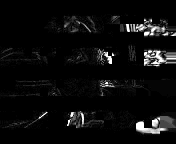
\includegraphics[width=0.46\linewidth]{images/diffCarphoneInterleaved.png}
\label{fig-392-err}
}
\end{varwidth}}
\caption{Exemple de l'erreur présente dans la sous-séquence \#392 du jeu de
tests (Séquence~: Carphone, QP=16 BER=0.0032, FMO=Dispersé)}
\label{fig-392}
\end{figure}

\begin{figure}[htb]
\fbox{\begin{varwidth}{\textwidth}\centering
\subfigure[Trame erronée]{
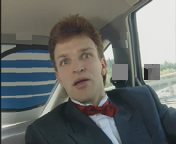
\includegraphics[width=0.46\linewidth]{images/badCarphoneDispersed.png}
\label{fig-1752-bad}
}
\subfigure[Erreur (amplifiée)]{
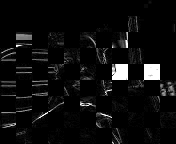
\includegraphics[width=0.46\linewidth]{images/diffCarphoneDispersed.png}
\label{fig-1752-err}
}
\end{varwidth}}
\caption{Exemple de l'erreur présente dans la sous-séquence
\#1752 du jeu de tests (Séquence~: Carphone, QP=16 BER=0.0032, FMO=Entrelacé)}
\label{fig-1752}
\end{figure}

Notre banc d'essai est constitué d'un jeu de tests de 2720 sous-ensembles de
trames, Plus précisément, nous avons 1360 trames dispersées et 1360 trames
entrelacées. Dans la prochaine section, ce banc d'essai servira à déterminer la
résilience du décodeur inclus dans le \ltCodec. À la
section~\ref{sec-ApprocheSelective}, il sera utilisé pour valider nos approches
sélectives de détection et de dissimulation d'erreur.

\end{section}

\begin{section}{Analyse de la résilience aur erreurs du décodeur de référence H.264}
\label{sec-ResilienceDecodeur}
Dans certaines conditions, le décodeur fournit avec le \ltCodec~réussi à décoder
des séquences binaires corrompues. Cette découverte, initiatrice de notre effort
de recherche, fut réalisée très tôt dans nos expérimentations.  Nous définissons
un décodage réussi comme~: l'opération de décoder une tranche corrompue sans
causer de défaillances \ang{crash} chez le décodeur, sans pour autant garantir
l'intégrité du contenu résultant. En d'autres mots, l'image issue du décodage
d'une tranche corrompue va souvent contenir de la dégradation visuelle (voir
figures \ref{fig-726-bad}, \ref{fig-392-bad} et \ref{fig-1752-bad}). Le taux de
décodages réussis varie, non seulement selon le taux d'erreur binaire appliqué à
la séquence, mais aussi à l'égard du paramètre de quantification (QP) utilisé
lors de l'encodage. Ceci s'explique par le fait qu'un QP plus faible force
l'encodeur à utiliser plus de bits pour encoder une trame; et plus il y a de
bits sujets à erreur et plus la probabilité de corruption de la trame augmente.

\begin{figure}[htb]
\fbox{\begin{varwidth}{\textwidth}\centering
\subfigure[Ordonnacement dispersé]{
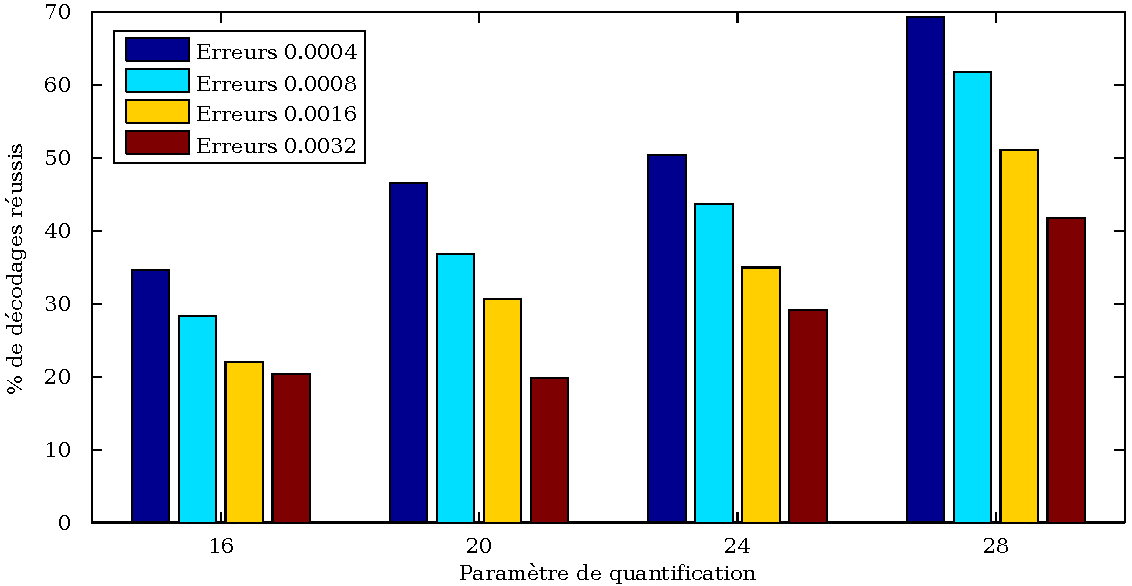
\includegraphics[width=0.97\linewidth]{images/decodingDispersed.pdf}
}\\
\subfigure[Ordonnacement entrelacé]{
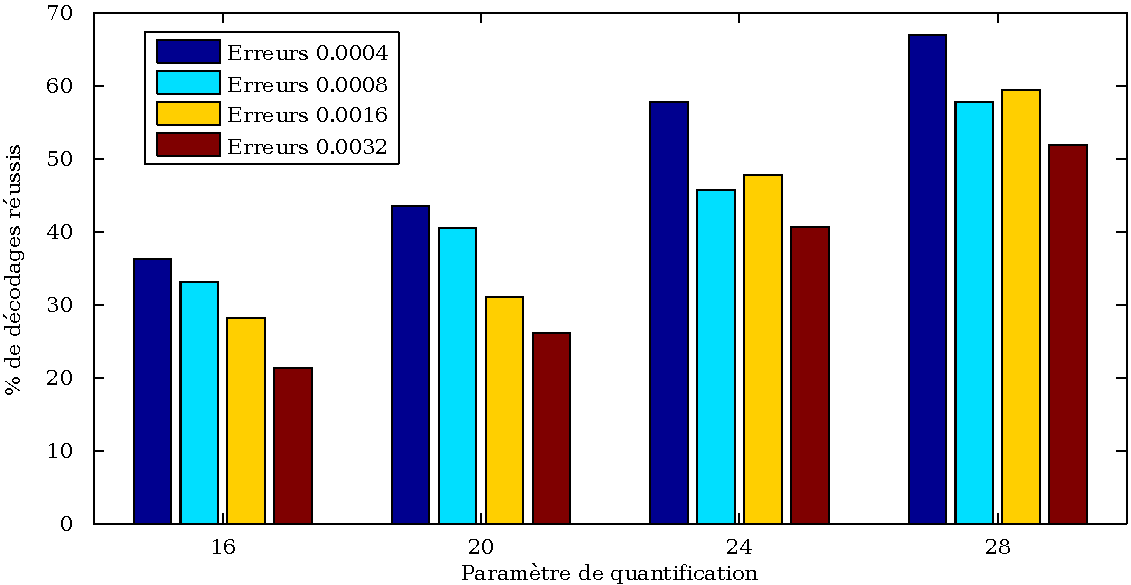
\includegraphics[width=0.97\linewidth]{images/decodingInterleaved.pdf}
}
\end{varwidth}}
\caption{Histogrammes des pourcentages de décodages réussis en fonction du
paramètre de quantification utilisé lors de l'encodage ainsi que du taux
d'erreurs sur les bits (BER). }
\label{fig-Decodings}
\end{figure}

Les histogrammes de la \fig{fig-Decodings} présentent les taux de décodages
réussis observés en fonction des paramètres de quantification et du taux
d'erreurs sur les bits présents dans notre jeu de tests. Ces taux sont
intéressants, car ils confirment que le décodage des données corrompues peut
avoir un taux de réussite allant de 20~\% à 70~\%, selon les conditions. On peut
concevoir une stratégie de résilience à l'erreur, où une prochaine génération de
décodeurs seraient en mesure d'effectuer une tentative de décodage d'une tranche
corrompue, dans un environnement contrôlé (possiblement un second décodeur),
afin de contrer l'impact d'une défaillance.

\begin{figure}[htb]
\fbox{\begin{varwidth}{\textwidth}\centering
\subfigure[Trame Corrompue]{
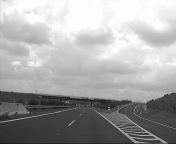
\includegraphics[width=0.30\linewidth]{images/ErrorFrame.png}
\label{fig-ErrorFrame}
}
\subfigure[Différentiel de \subref{fig-ErrorFrame} et la trame non-erronée]{
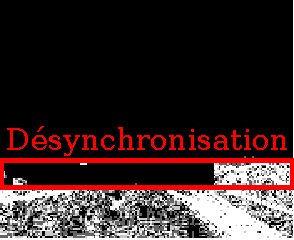
\includegraphics[width=0.30\linewidth]{images/Desync.pdf}
\label{fig-Desync}
}
\subfigure[Différentiel de \subref{fig-ErrorFrame} et la trame précédente]{
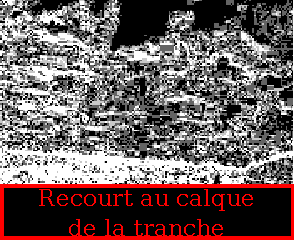
\includegraphics[width=0.30\linewidth]{images/Revert.pdf}
\label{fig-Revert}
}
\end{varwidth}}
\caption{Exemple du comportement du décodeur. En \subref{fig-Desync}, le
différentiel de \subref{fig-ErrorFrame}, par rapport à la trame codée/décodée
sans erreur, est utilisé pour démontrer la désynchronisation. Le différentiel
entre \subref{fig-ErrorFrame} et la trame précédente permet de démontrer, en
\subref{fig-Revert}, l'utilisation du calque de tranche.}
\label{fig-DecoderBehavior}
\end{figure}

Lors du décodage d'une tranche corrompue, le décodeur inclus dans le
\ltCodec~fait la transition entre trois états distincts. Le résultat de ceux-ci
est illustré à la \fig{fig-DecoderBehavior}. Le premier état est celui du
décodage des bits de la tranche corrompue situés avant l'erreur. Cet état est
équivalant au décodage normal d'une trame. Il est illustré par la partie
supérieure, tout en noir (signifiant l'absence de différence), du
différentiel~\subref{fig-Desync} de la \fig{fig-DecoderBehavior}.

Par la suite, le décodeur décode le premier bit corrompu. Ceci cause une
désynchronisation des codes binaires de l'encodage entropique. Même si les
autres bits de la séquence sont valides, la désynchronisation fait en sorte
qu'ils sont associés à la mauvaise valeur dans la table de référence CAVLC. Le
décodeur interprète ces mauvaises valeurs; ce qui entraîne une dégradation
visuelle dans l'image. Cette dégradation peut se manifester fortement comme
c'est le cas dans l'image de la \fig{fig-726-bad} ou être presque imperceptible,
comme c'est le cas dans la \fig{fig-ErrorFrame}. Afin de mieux voir la
dégradation visuelle de la \fig{fig-ErrorFrame}, elle est encadrée à la
\fig{fig-Desync}. C'est dans ce second état que le décodeur est le plus
vulnérable aux défaillances.

Le second état se termine lorsque le décodeur cesse d'insérer de la dégradation
visuelle dans l'image et utilise le contenu provenant de la tranche précédente.
Ce changement est illustré en~\ref{fig-Revert}. Ici, on suppose que le décodeur
est complètement désynchronisé, il ne sait que faire de ce qu'il décode, il
applique donc le contenu des blocs précédents, ce qui, grâce à la corrélation
temporelle, est le contenu de remplacement correct, s'il y a absence de
mouvement. De plus, notons que dans l'image~\ref{fig-ErrorFrame}, il y a très
peu d'effet de blocs causés par la désynchronisation. Ceci est dû au filtre
antiblocs. Lorsqu'il est appliqué sur la trame, il va identifier et lisser les
effets de blocs. Ceci explique aussi pourquoi, à la \fig{fig-392-bad}, l'erreur
se répand à la tranche non erronée. Dans ce cas, le filtre antiblocs lisse le
bloc erroné, ce qui répand l'erreur dans les blocs avoisinants.

\end{section}

\begin{section}{Analyse de l'approche sélective}
\label{sec-ApprocheSelective}
Comme démontré dans la section précédente, l'image résultante d'une tranche
corrompue peut souvent être décodée. Cependant, celle-ci possède, dû à la
désynchronisation du décodeur lors du décodage, une dégradation visuelle plus ou
moins importante. Elle peut toutefois être utilisée pour guider un algorithme de
dissimulation d'erreur grâce à un nouveau type d'algorithme permettant la
détection de la dégradation visuelle proposé dans ce mémoire.

L'algorithme de détection basé la mesure des effets de blocs compensés par le
mouvement (MCB), présenté dans cet ouvrage, permet la détection d'un type de
dégradation visuelle, celui causant des effets de blocs absents de la trame
précédente. La prémisse de notre approche sélective est de déterminer entre le
calque de la tranche (\fig{fig-726-sc}) et la tranche corrompue
(\fig{fig-726-bad}), celui qui produirait la meilleure dissimulation (c.-à-d.
produisant le meilleur PSNR par rapport à la trame de référence). Cette
opération peut être accomplie à deux niveaux~: celui de la tranche, à l'aide du
SDMCB, ou des blocs, avec le MCB. Nous allons tout d'abord présenter la
configuration de notre banc de tests pour mesurer l'approche sélective. Par la
suite, la sous-section~\ref{sec-AnalyseSDMCB} présente les résultats obtenus
avec le SDMCB et les résultats du MCB sont présentés à la
sous-section~\ref{sec-AnalyseMCB}.
\LT{MCB, SDMCB et le PSNR sont présentés dans des séctions précédentes.}

\begin{figure}[htb]
\fbox{\centering
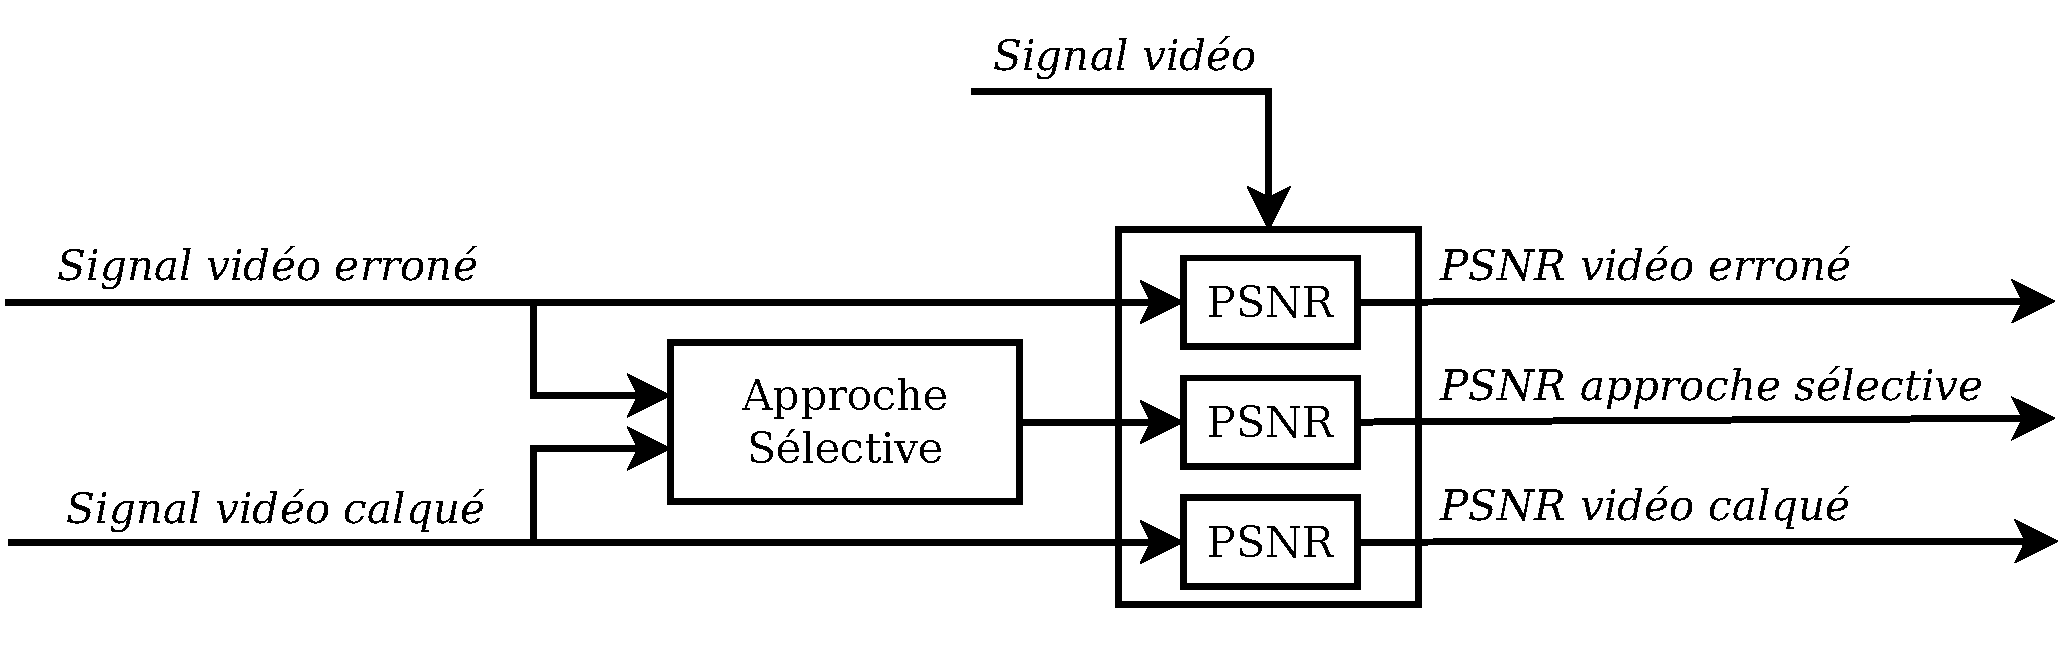
\includegraphics[width=0.75\linewidth]{images/SelectiveSetup.pdf}
}
\caption{Partie~2 de la Figure~\ref{fig-EncoderDecoder}. Configuration du banc
d'essai pour mesurer l'approche sélective basée SDMCB et MCB.}
\label{fig-SelectiveSetup}
\end{figure}

Tout d'abord, à l'aide du PSNR comme discriminant, nous mesurons la distribution
des meilleures dissimulations, entre le calque de la tranche et la tranche
corrompue. La \fig{fig-SelectiveSetup} démontre la configuration élaborée pour
obtenir ces mesures. On y constate que le PSNR est mesuré par rapport au signal
vidéo de référence et qu'il est mesuré pour l'image résultante du décodage de la
tranche corrompue, le candidat de dissimulation basée sur le calque de la
tranche et le résultat des approches sélectives basées sur le SDMCB et MCB.

Les résultats mesurés sur le banc de tests proposé sont présentés à la
\fig{fig-ScVsErroneous}. On y remarque une importante quantité de trames et de
blocs erronés qui possèdent un PSNR supérieur aux calques de trames. Cela
s'explique par le fait que, dans ces cas, la dégradation visuelle engendrée par
la désynchronisation du décodeur est moins importante que la variation
temporelle par rapport à la trame précédente; ce qui pénalise
 le calque de tranche. En lien avec les trois états d'un décodeur
traitant une tranche corrompue, nous pouvons conclure que dans l'état~1, la
tranche endommagée va produire un meilleur résultat que le calquage de la
tranche. Dans l'état~2, la tranche endommagée va produire un résultat inférieur
à la tranche calquée. Finalement, à l'état~3, les deux sont équivalents. La
proportion de blocs compris dans les états~1 et 2, l'intensité de la dégradation
produite par le décodeur ainsi que la variation temporelle par rapport à la
trame précédente sont les facteurs qui déterminent laquelle des deux trames
constituera la meilleure dissimulation.

\begin{figure}[htb]
\fbox{\begin{varwidth}{\textwidth}\centering
\subfigure[Distribution des trames corrompues (ronds rouges) par rapport aux
trames calquées (ligne bleue)]{
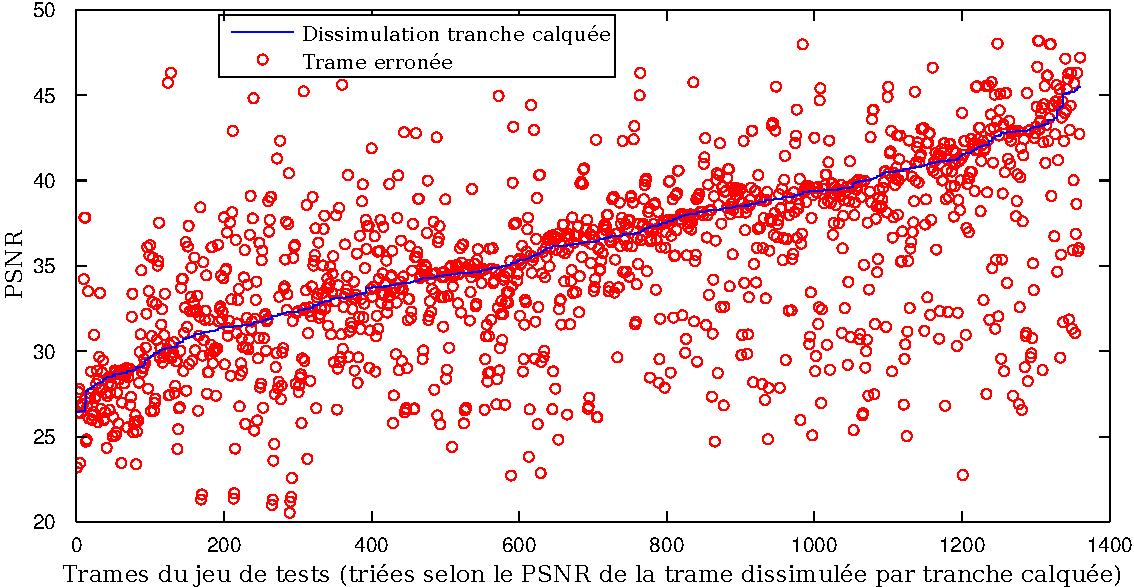
\includegraphics[width=0.97\linewidth]{images/scVsErroneous.pdf}
\label{fig-scVsErroneous}
}\\
\subfigure[Distribution des blocs issus des trames corrompues (ronds magenta)
par rapport aux blocs issus des trames calquées (ligne noire). À des fins de
visualisation, seulement un bloc sur dix est affiché.]{
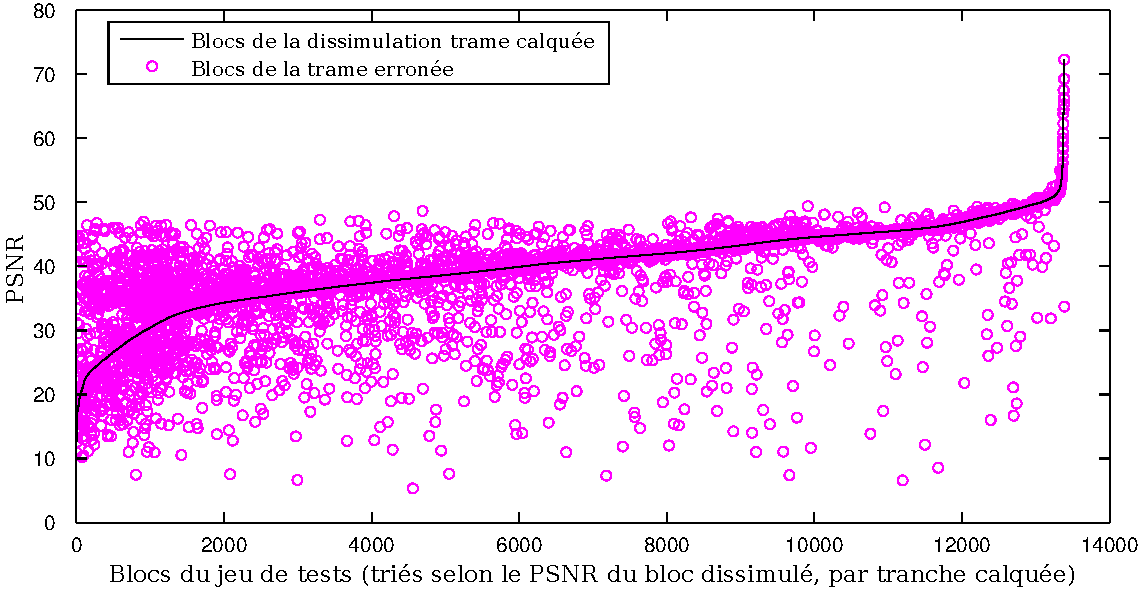
\includegraphics[width=0.97\linewidth]{images/ScVsErroneousBlocks.pdf}
\label{fig-scVsErroneousBlocks}
}
\end{varwidth}}
\caption{Visualisation de la distribution des valeurs du PSNR de la trame
erronée et de la dissimulation par tranche calquée.}
\label{fig-ScVsErroneous}
\end{figure}

Plus précisément, les mesures obtenues de notre banc d'essai nous permettent de
conclure que l'image résultante du décodage de la tranche corrompue offre un
PSNR plus élevé dans 44~\% des cas pour l'ordonnancement dispersé et 49~\% pour
l'entrelacé. Pour ces trames, on observe respectivement des gains moyens de
2.12~dB et 1.68~dB par rapport à leurs trames équivalentes calquées. De manière
similaire, les blocs issus de trames corrompues sont supérieurs dans 42~\% des
cas pour l'ordonnancement dispersé et 49~\% pour l'entrelacé. Ces blocs
produisent, pour les approches d'ordonnancement précédentes, des gains moyens de
1.44~dB et 1.02~dB.

Nous avons démontré, non seulement, qu'il est possible de réussir à décoder des
tranches erronées. Mais aussi qu'une quantité importante des images résultantes
exhibent une fidélité visuelle supérieure au calque de cette tranche (approche
couramment employée par le décodeur fourni avec le \ltCodec).

\begin{subsection}{Approche sélective SDMCB}
\label{sec-AnalyseSDMCB}
Maintenant, toujours avec la même configuration du banc de test, mesurons
l'aptitude du SDMCB à identifier le meilleur candidat entre la trame corrompue
et la dissimulation par tranche calquée. Pour ce faire, nous allons utiliser une
taille de bloc $B=16$ (vu notre indépendance au train de bits, nous ne
connaissons pas la taille exacte des blocs) et un seuil d'effet de bloc $T_b =
5000$.

\begin{figure}[htb]
\fbox{\begin{varwidth}{\textwidth}\centering
\subfigure[Ordonnancement dispersé]{
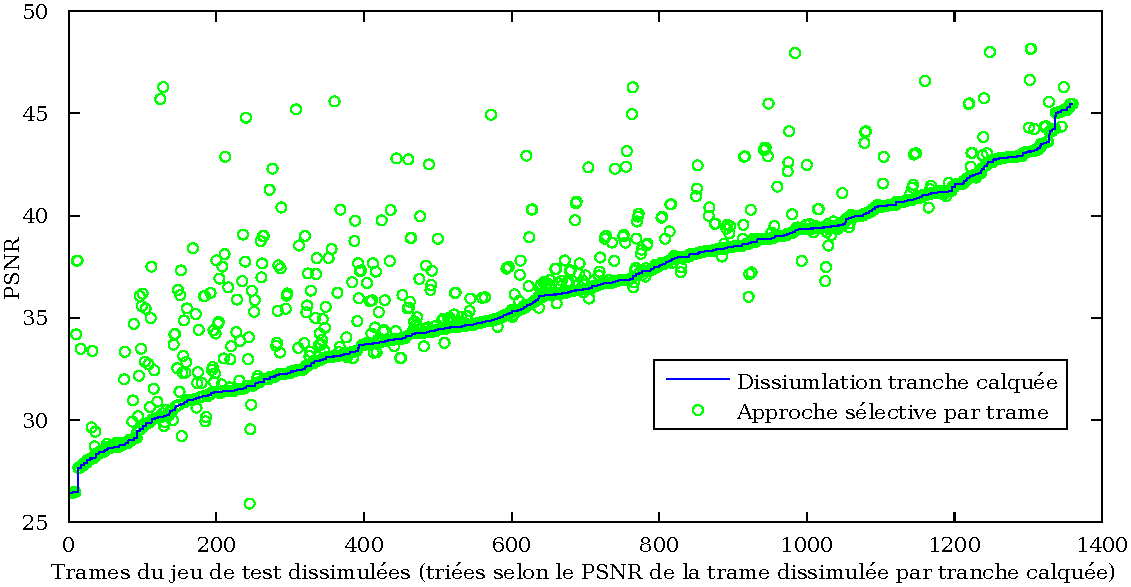
\includegraphics[width=0.97\linewidth]{images/selectiveSliceCopyDispersed.pdf}
\label{fig-sliceCopyDispersed}
}\\
\subfigure[Ordonnancement entrelacé]{
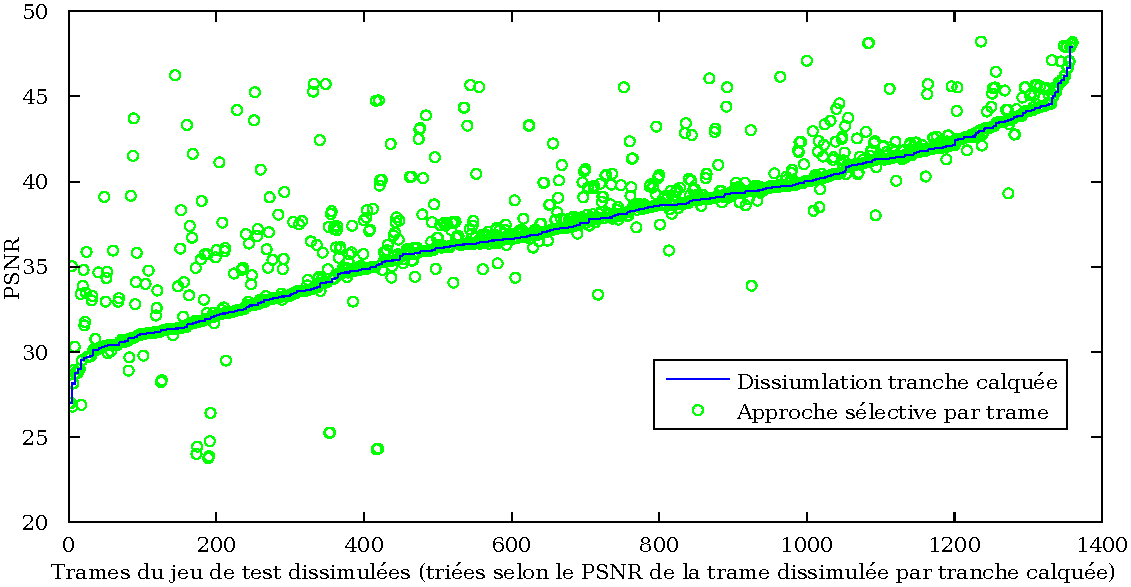
\includegraphics[width=0.97\linewidth]{images/selectiveSliceCopyInterleaved.pdf}
\label{fig-sliceCopyInterleaved}
}
\end{varwidth}} 
\caption{Visualisation de la distribution du PSNR de l'approche sélective basée
sur SDMCB (ronds verts) à l'égard de la dissimulation par tranche calquée (ligne
bleue).}
\label{fig-SelectiveSliceCopy}
\end{figure}

Les résultats obtenus sont présentés à la \fig{fig-SelectiveSliceCopy}. La
\fig{fig-sliceCopyDispersed} témoigne que l'approche sélective, dans le cadre
d'un ordonnancement dispersé, fait le bon choix dans 81~\% des cas. Pour
ceux-ci, un gain moyen de 1.98~dB est mesuré, tandis que pour l'ensemble de la
séquence le gain moyen est de 0.72~dB. Les choix de l'approche sélective offrent
un PSNR supérieur aux trames dissimulées par calquage de tranche dans 31~\% des
cas. Pour la \fig{fig-sliceCopyInterleaved}, la bonne trame est choisie dans
86~\% des cas, résultant dans un gain moyen de 1.24~dB pour celles-ci. Sur
l'ensemble des trames, le gain moyen est de 0.65~dB et un PSNR supérieur au
calquage de trame est obtenu dans 43~\% des cas.

\end{subsection}
\begin{subsection}{Approche sélective MCB}
\label{sec-AnalyseMCB}
Le niveau de granularité plus fin de l’approche sélective MCB est son attrait
principal. En remplaçant uniquement les blocs endommagés, on maximise l’usage
des données correctement décodées.

Sans altérer la configuration de notre banc de test, nous mesurons l'aptitude du
MCB à identifier le meilleur bloc candidat entre ceux provenant de la trame
corrompue et ceux de la dissimulation par tranche calquée. Pour ce faire, nous
allons utiliser une taille de bloc $B=16$ et un seuil d'effet de bloc $T_b =
5000$.

\begin{figure}[htb]
\fbox{\begin{varwidth}{\textwidth}\centering
\subfigure[Ordonnancement dispersé]{
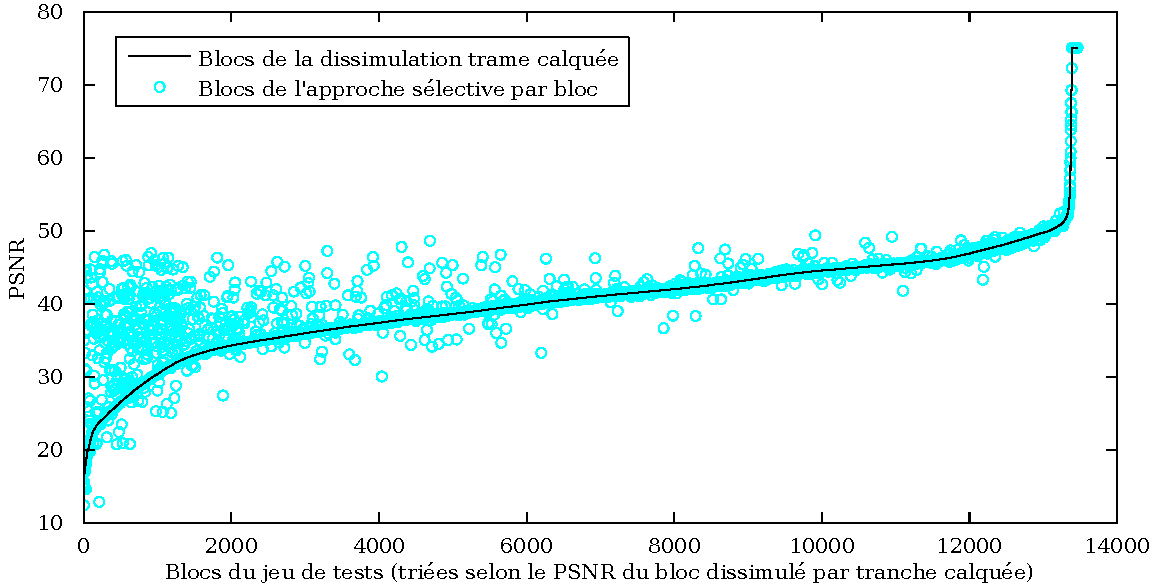
\includegraphics[width=0.97\linewidth]{images/SelectiveSliceCopyBlocksDispersed.pdf}
\label{fig-selectiveSliceCopyBlockDispersed}
}\\
\subfigure[Ordonnancement entrelacé]{
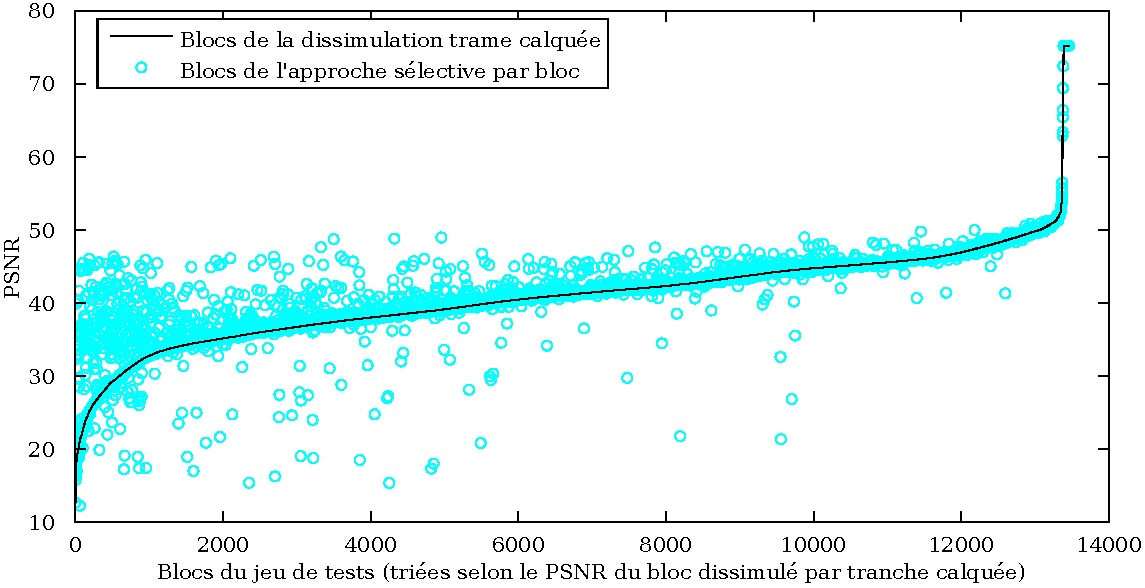
\includegraphics[width=0.97\linewidth]{images/SelectiveSliceCopyBlocksInterleaved.pdf}
\label{fig-selectiveSliceCopyBlockInterleaved}
}
\end{varwidth}}
\caption{Visualisation de la distribution du PSNR issue des blocs résultants de
l'approche sélective basée sur MCB (ronds verts) à l'égard de ceux produits par
la dissimulation par tranche calquée (ligne bleue).}
\label{fig-SelectiveSliceCopyBlocks}
\end{figure}

Les résultats obtenus sont présentés à la \fig{fig-SelectiveSliceCopyBlocks}. La
\fig{fig-selectiveSliceCopyBlockDispersed} démontre que l'approche sélective MCB
choisit le bon bloc dans 88~\% de cas. Ce qui produit un gain moyen de 0.86~dB
sur l'ensemble des trames avec un ordonnancement de type dispersé. Pour
l'ordonnancement entrelacé (\fig{fig-selectiveSliceCopyBlockInterleaved}),
l'approche sélective MCB effectue le bon choix dans 91~\% des cas, permettant un
gain moyen de 0.69~dB.

\end{subsection}

À l'aide de la \fig{fig-FrameDistribution}, nous sommes en mesure d'analyser la
distribution des PSNR résultants~: de la trame erronée, de la dissimulation par
tranche calquée et des approches sélectives. Cette figure expose la variation du
nombre de trames selon des intervalles de 5~dB de PSNR. Ces intervalles
s'étalent de 20~dB à 50~dB, permettant ainsi de visualiser la variation de la
qualité visuelle issue de chaque approche. Commençons l'analyse en soulignant la
présence d'une importante quantité de trames erronées dans les intervalles de
faible qualité, où le PSNR est inférieur à 30 (les intervalles centrés autour de
20 et 25). Pour ces intervalles, nous constatons, autant dans l'histogramme de
la \fig{fig-SelectiveHistDispersed} que \ref{fig-SelectiveHistInterleaved}, que
la majorité de ces trames sont dissimulées par le calquage de tranche et les
approches sélectives. Poursuivons l'analyse des approches sélectives avec le
constat suivant, pour l'intervalle centré autour de 30~dB, le nombre de trames
liées aux approches sélectives est inférieur à celui lié à la dissimulation par
tranche calquée. Cette observation n'est pas due à une perte de qualité, mais
bien à une augmentation de la qualité, car on retrouve ces trames dans les
intervalles supérieurs. Pour ces intervalles, les approches sélectives
produisent un plus grand nombre de trames que la dissimulation par tranche
calquée. Grâce à ces observations, nous sommes en mesure de conclure que les
approches sélectives produisent de meilleurs résultats en exploitant les trames
erronées de haute qualité visuelle, tout en évitant les trames erronées de
mauvaise qualité. En ce qui a trait à la comparaison des approches sélectives,
l'approche sélective MCB offre un plus grand nombre de trames de qualité
visuelle pour les intervalles de 35~dB et 40~dB vis-à-vis SDMCB. Cependant,
cette dernière se reprend dans l'intervalle de 45~dB. Cette reprise est
attribuée au fait que le remplacement de blocs sporadique dans une trame peut
engendrer une perte de qualité causée par le mauvais arrimage des valeurs de
pixels en frontière de bloc. Cette légère dégradation réduit le nombre de trames
de très haute qualité. Toutefois à des niveaux de 40dB et plus, la différence de
qualité est souvent imperceptible.

\begin{figure}[htb]
\fbox{\begin{varwidth}{\textwidth}\centering
\subfigure[Ordonnancement dispersé]{
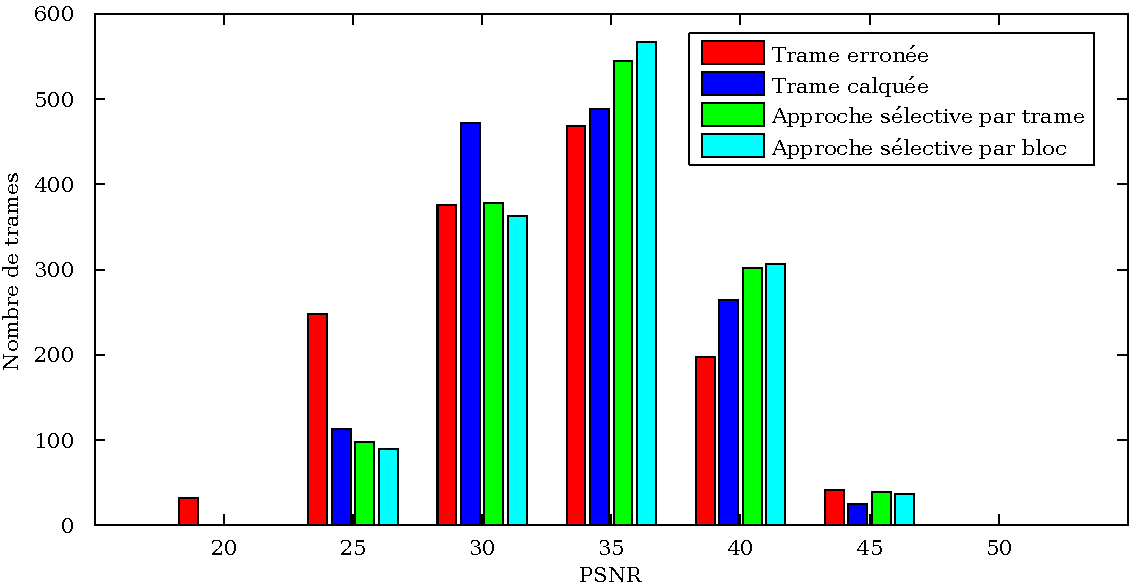
\includegraphics[width=0.97\linewidth]{images/SelectiveHistDispersed.pdf}
\label{fig-SelectiveHistDispersed}
}\\
\subfigure[Ordonnancement entrelacé]{
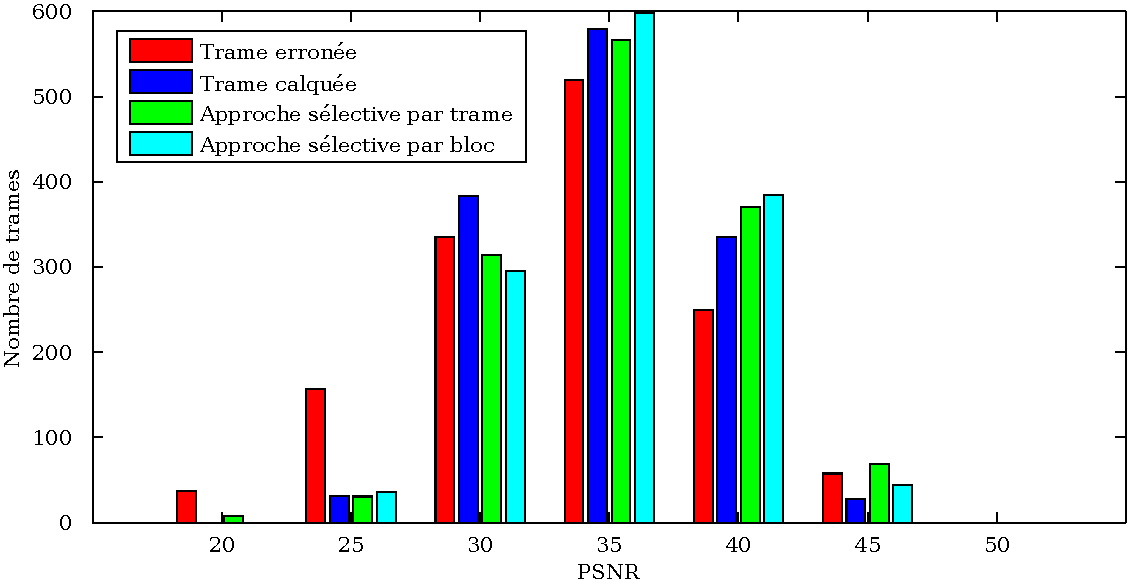
\includegraphics[width=0.97\linewidth]{images/SelectiveHistInterleaved.pdf}
\label{fig-SelectiveHistInterleaved}
}
\end{varwidth}}
\caption{Histogrammes des PSNR des trames, avec des intervalles de 5~dB, centrés
à chaque incrément de 5~dB, à partir de 20~dB. Les trames considérées sont
celles résultantes~: du décodage de la trame erronée (rouge), du calquage de
tranche (bleu), de l'approche sélective par tranche (vert) ainsi que
l'approche sélective par bloc (cyan).} 
\label{fig-FrameDistribution}
\end{figure}

\begin{table}[!htb]
\caption{Résumé du PSNR moyen obtenu par les diverses approches présentées dans
cette section sur le jeu de tests.}
\label{tab-ResumeSelectif}
\small
\centering
\begin{tabular}{| l | c | c |}
 \hline
 \textbf{Approche} & \textbf{PSNR Moyen}& \textbf{PSNR Moyen}\\
 &\textbf{dispersé (dB)}&\textbf{entrelacé (dB)}\\
 \hline
 Encodée (sans erreur) & 41.218222 & 41.200377\\
  \hline
 Sélective par bloc (avec référence) & 37.689039 & 38.528986\\
  \hline
 Sélective par tranche (avec référence) & 37.117712 & 38.082769\\
  \hline
 Sélective MCB & \textbf{37.034840} & \textbf{37.951004}\\
  \hline
 Sélective SDMCB & \textbf{36.901414} & \textbf{37.911514}\\
  \hline
 Dissimulation tranche calquée & 36.179630 & 37.263033\\
  \hline
 Trame corrompue & 35.068784 & 36.075526\\
 \hline   
\end{tabular}
\end{table}

\SC{Il faut présenter et analyser le tableau 1.1. Il manque aussi une petite
conclusion au chapitre}

\end{section}

\bibliographystyle{bibETS}
\bibliography{resultats}

\end{chapter}

\end{document}